\documentclass[conf]{new-aiaa}
%\documentclass[journal]{new-aiaa} for journal papers
\usepackage[utf8]{inputenc}

\usepackage{graphicx}
\usepackage{amsmath}
\usepackage[version=4]{mhchem}
\usepackage{listings}
\usepackage{color}
\usepackage{siunitx}
\usepackage{longtable,tabularx}
\usepackage{subcaption}
\usepackage{cleveref}
\usepackage{appendix}
\setlength\LTleft{0pt}

\title{Solution of 1D heat conduction equation with constant source \\ using \\ Spectral Methods}

% \author{Ramkumar S. \footnote{SC22M007, M.Tech., Aerospace AFM }}
% \affil{SC22M007, M.Tech. Aerospace - Aerodynamics and Flight Mechanics}
\author{Ramkumar S.}


\definecolor{mygreen}{rgb}{0,0.6,0}
\definecolor{mygray}{rgb}{0.5,0.5,0.5}
\definecolor{mymauve}{rgb}{0.58,0,0.82}

\lstset{
  backgroundcolor=\color{white},   % choose the background color; you must add \usepackage{color} or \usepackage{xcolor}; should come as last argument
  basicstyle=\footnotesize,        % the size of the fonts that are used for the code
  breakatwhitespace=false,         % sets if automatic breaks should only happen at whitespace
  breaklines=true,                 % sets automatic line breaking
  captionpos=b,                    % sets the caption-position to bottom
  commentstyle=\color{mygreen},    % comment style
  deletekeywords={...},            % if you want to delete keywords from the given language
  escapeinside={\%*}{*)},          % if you want to add LaTeX within your code
  extendedchars=true,              % lets you use non-ASCII characters; for 8-bits encodings only, does not work with UTF-8
  firstnumber=0001,                % start line enumeration with line 1000
  frame=single,                    % adds a frame around the code
  keepspaces=true,                 % keeps spaces in text, useful for keeping indentation of code (possibly needs columns=flexible)
  keywordstyle=\color{blue},       % keyword style
  language=Octave,                 % the language of the code
  morekeywords={*,...},            % if you want to add more keywords to the set
  numbers=left,                    % where to put the line-numbers; possible values are (none, left, right)
  numbersep=5pt,                   % how far the line-numbers are from the code
  numberstyle=\tiny\color{mygray}, % the style that is used for the line-numbers
  rulecolor=\color{black},         % if not set, the frame-color may be changed on line-breaks within not-black text (e.g. comments (green here))
  showspaces=false,                % show spaces everywhere adding particular underscores; it overrides 'showstringspaces'
  showstringspaces=false,          % underline spaces within strings only
  showtabs=false,                  % show tabs within strings adding particular underscores
  stepnumber=2,                    % the step between two line-numbers. If it's 1, each line will be numbered
  stringstyle=\color{mymauve},     % string literal style
  tabsize=2,                       % sets default tabsize to 2 spaces
  % title=\lstname                 % show the filename of files included with \lstinputlisting; also try caption instead of title
}

\begin{document}

\maketitle

\begin{abstract}
    The solution of 1D heat conduction equation with constant boundary temperatures
    and constant heat source was done using spectral methods. The results were
    compared with analytical solution for a range of number of terms in the
    basis function series and the observation was recorded. Modern Fortran code was
    developed for the solution of equations and a Python3 script was made for
    the post-processing of the results.
\end{abstract}

\section{Problem definition}
\par The present problem is described in the \cref{problem_description}.
\vspace{1cm}
\begin{figure}[!h]
   \center
    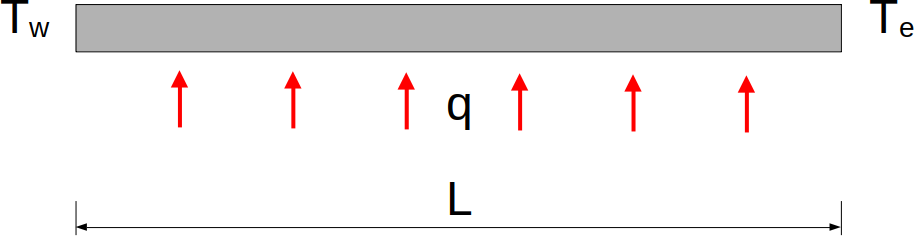
\includegraphics[scale=0.2]{supportingFiles/schematic.png}
    \caption{problem definition}
    \label{problem_description}
\end{figure}

\par A rod of length L is taken with the constant temperatures at both ends
as $T_w$ and $T_e$, and with constant heat source, $q$. The heat conduction
of the material is taken to be $k$. The governing equation for the present
problem is given in \cref{govEqn}.

\begin{align}
    k\frac{\partial^2 T}{\partial x^2} + q = 0 \label{govEqn}
\end{align}

\par The analytical solution for the present problem is given in \cref{analyticalEqn}
for \(\displaystyle{0 \le x \le L}\).

\begin{align}
    T_x = -\frac{q x^2 }{2 k} + \frac{1}{L}\left(T_e-T_w + \frac{q L^2}{2 k}\right)x + T_w \label{analyticalEqn}
\end{align}

\section{Solution methodology}
The present problem was solved using spectral methods. The advantages of
spectral methods over finite-difference can be found in the literature, at the
same time, the disadvantage of spectral methods is its limited applicability
to problems with simpler domain and boundary conditions. Moreover, the solution
to the governing equation must be smooth, i.e. no discontinuities like shocks,
for the spectral method to give better results. The assumed solution to the
governing equation is given in \cref{assumedSolution}.
\begin{align}
    T_x = T_w + \frac{T_e - T_w}{L}x + \sum_{n=1}^N a_n sin\left(\frac{n\pi}{L}x\right) \label{assumedSolution}
\end{align}

\par Here, the basis function is taken as sine function, and the \cref{assumedSolution}
should be made such that it satisfies the boundary condition as given below.
\begin{align*}
    \phi_n &= sin\left(\frac{n \pi}{L}x\right) \\
    T_{(x=0)} &= T_w \\
    T_{(x=L)} &= T_e
\end{align*}

\par Differentiating \cref{assumedSolution} twice gives, \cref{derivativeEqn}
\begin{align}
    \frac{\partial^2 T}{\partial x^2} &= - \sum_{n=1}^N a_n \left(\frac{n \pi}{L}\right)^2 sin \left(\frac{n \pi}{L}x\right) \label{derivativeEqn}
\end{align}

\par Substituting the \cref{derivativeEqn} in \cref{govEqn} gives the residual equation \cref{residualEqn} below.
\begin{align}
    r  &= - \sum_{n=1}^N a_n \left(\frac{n \pi}{L}\right)^2 sin \left(\frac{n \pi}{L}x\right)  + q = 0 \label{residualEqn}
\end{align}

\par Following Galerkin method for weighted residuals, the governing equation to
determine the unknown coefficients $a_n$ is given in \cref{an_eqn}.

\begin{align}
    \int_0^L r \phi_i dx = 0 \label{an_eqn} \\
    \int_0^L \left(- \sum_{n=1}^N a_n \left(\frac{n \pi}{L}\right)^2 sin \left(\frac{n \pi}{L}x\right)  + q \right)  sin\left(\frac{i\pi}{L}x\right) = 0 \nonumber
\end{align}

\par Here the subscripts i and n are like nested loops with same range, hence taking advantage of orthogonal basis
functions, the derived final expression for the coefficients is given in \cref{an_expression}.
\begin{align}
    a_n &= \frac{2 q}{k} \frac{L^2}{\left(n \pi\right)^3} \left(1 - \left(-1\right)^n\right) \label{an_expression}
\end{align}

\par The \cref{an_expression} gives the coefficient values till N series terms.
The order of accuracy of the solution depends on the number of terms in the
series taken. Substituting the computed $a_n$ values in the \cref{assumedSolution}
will give the temperature distribution.

\section{Results}
\par The results obtained for different N series terms is given in \cref{results_figure},
along with the error percentage for each case. It can be seen that the
error percentage of the results obtained in comparison with analytical solution,
reduces as the number of terms in the sine series increases. The solution
matched exactly with the analytical solution for the terms count of N = 40.

\begin{figure}[!htb]
    \centering
    \begin{subfigure}{0.45\textwidth}
        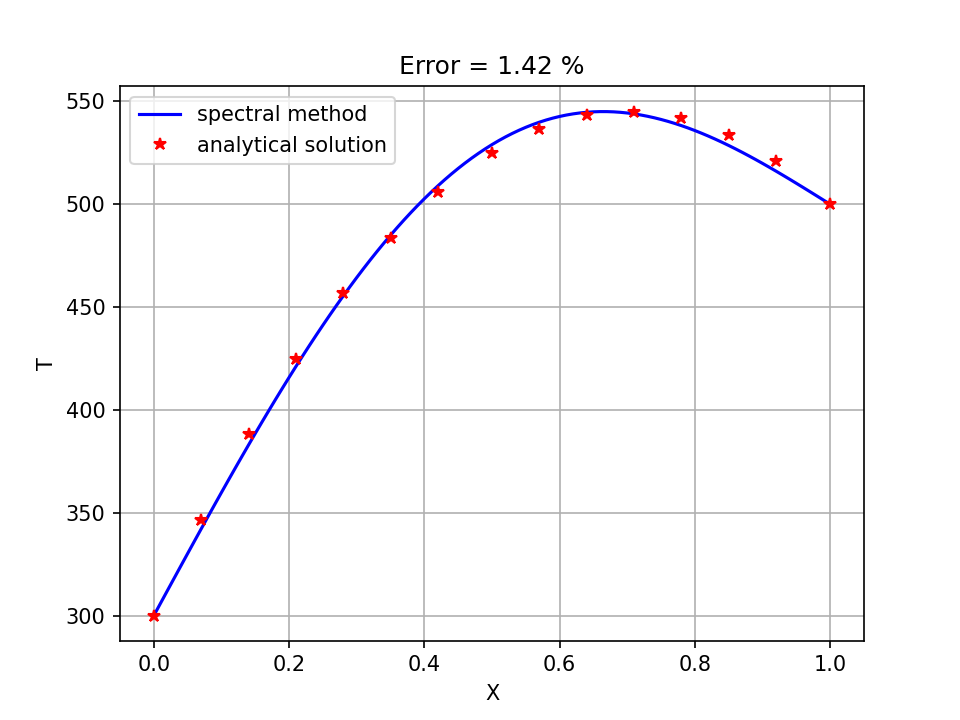
\includegraphics[width=\textwidth]{supportingFiles/output_N_1.png}
        \label{N_1}
        \caption{N = 1}
    \end{subfigure}
    \hfill
    \begin{subfigure}{0.45\textwidth}
        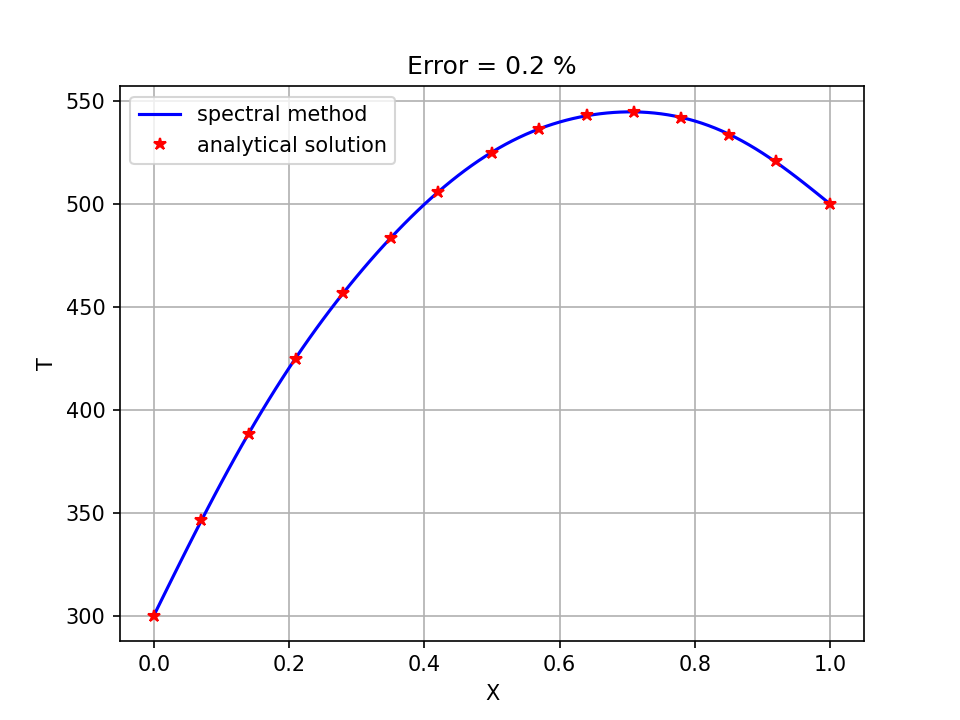
\includegraphics[width=\textwidth]{supportingFiles/output_N_5.png}
        \label{N_5}
        \caption{N = 5}
    \end{subfigure}
    \hfill
    \begin{subfigure}{0.45\textwidth}
        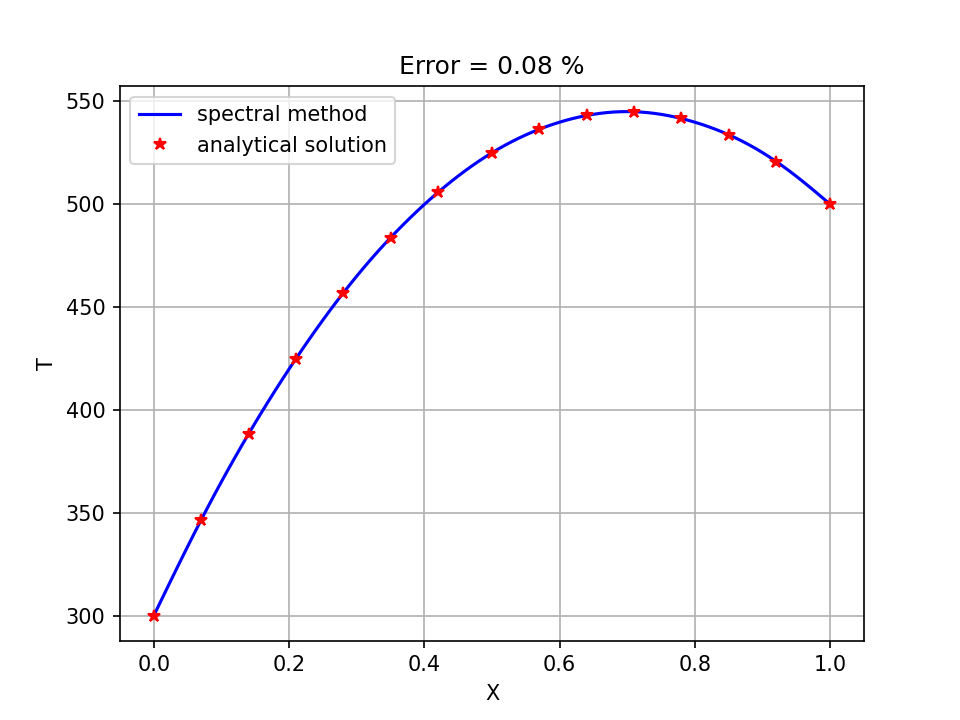
\includegraphics[width=\textwidth]{supportingFiles/output_N_10.png}
        \label{N_10}
        \caption{N = 10}
    \end{subfigure}
    \hfill
    \begin{subfigure}{0.45\textwidth}
        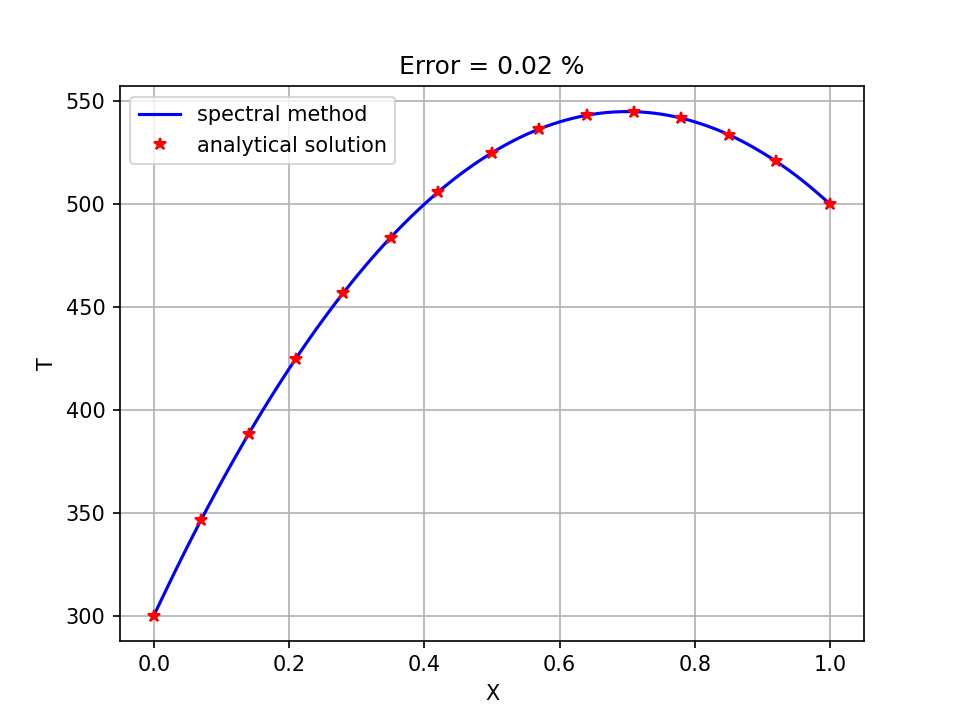
\includegraphics[width=\textwidth]{supportingFiles/output_N_20.png}
        \label{N_20}
        \caption{N = 20}
    \end{subfigure}
    \hfill
    \begin{subfigure}{0.45\textwidth}
        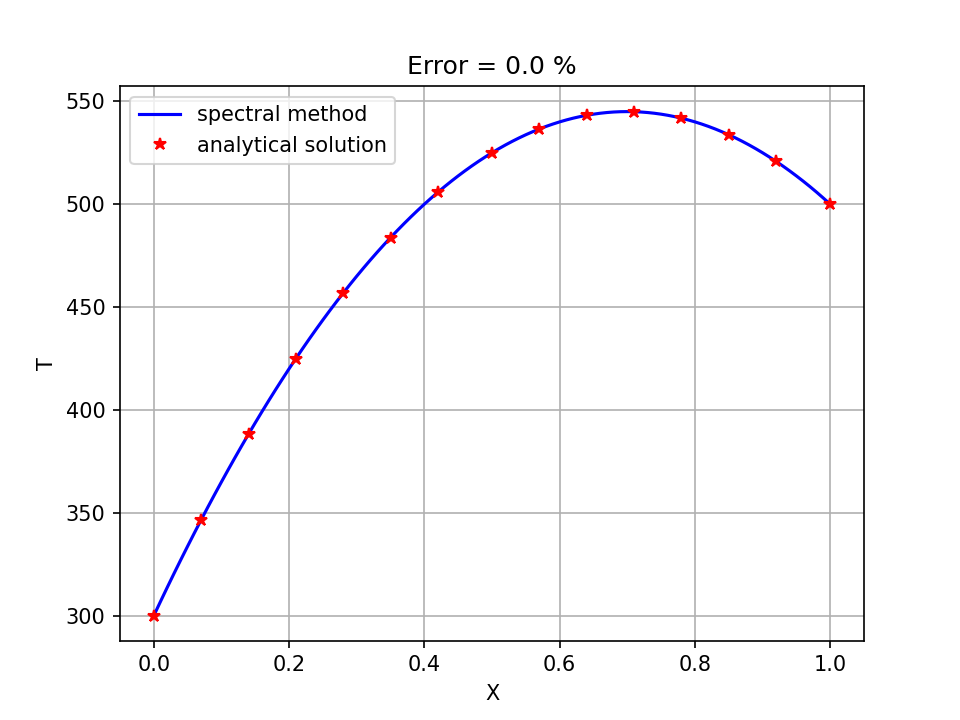
\includegraphics[width=\textwidth]{supportingFiles/output_N_40.png}
        \label{N_40}
        \caption{N = 40}
    \end{subfigure}
    \caption{variation of accuracy of the results computed using spectral methods}
    \label{results_figure}
\end{figure}

\section{Conclusion and future works}
The solution to 1D heat conduction equation with constant source terms and
boundary conditions was obtained successfully using the spectral methods.
The present work will be further extended to 2D heat conduction and later to
the solution of Euler/Navier Stokes equations for a driven cavity flow problem.

\par The FORTRAN program files and Python code of the present work is given in
\Cref{appendixA}.

% \begin{thebibliography}{2}
%     \bibitem{ref_1} Online Prandtl-Meyer expansion flow calculator; https://www.omnicalculator.com/physics/prandtl-meyer-expansion
%     \bibitem{ref_2} Michel A. Saad; Compressible fluid flow
% \end{thebibliography}

\pagebreak

\begin{appendices}
    \section{Appendix - FORTRAN and Python codes}\label{appendixA}
    This section contains the FORTRAN and Python codes used in the present work \\
    \par Below is the main FORTRAN program that solves the present problem.

    \lstinputlisting[language=Fortran]{supportingFiles/codes/main.f90}

    \par Below is the parameters FORTRAN file containing modules of computation parameters
    \lstinputlisting[language=Fortran]{supportingFiles/codes/parameters.f90}

    \par Below is the FORTRAN file containing the subroutines needed in the computations.
    \lstinputlisting[language=Fortran]{supportingFiles/codes/subroutines1.f90}

    \par Below is the Makefile that is used to compile and execute the program.
    \lstinputlisting[language=make]{supportingFiles/codes/Makefile}

    \par And below is the Python script used for plotting and error computation.
    \lstinputlisting[language=Python]{supportingFiles/codes/script.py}

\end{appendices}

\par
\center{**********}

\end{document}
